% Exam 1 Review -- Metropolis beamer slides
% Compile: pdflatex exam-1-review.tex (x2)
\documentclass[10pt,aspectratio=169]{beamer}

\usetheme{metropolis}
\metroset{block=fill, numbering=fraction, progressbar=frametitle}

\usepackage[T1]{fontenc}
\usepackage{amsmath, amssymb}
\usepackage{listings}
\usepackage{booktabs}
\usepackage{tikz}
\usepackage{pgfplots}
\pgfplotsset{compat=1.18}
\usetikzlibrary{arrows.meta, positioning, decorations.pathreplacing, calc}

% ---- colors -------------------------------------------------------------
\definecolor{mLightBlue}{HTML}{4C72B0}
\definecolor{mGreen}{HTML}{55A868}
\definecolor{mRed}{HTML}{C44E52}
\definecolor{mGray}{HTML}{BFBFBF}
\setbeamercolor{alerted text}{fg=mRed}

% ---- code style ---------------------------------------------------------
\lstdefinestyle{jl}{
  basicstyle=\ttfamily\footnotesize,
  keywordstyle=\color{mRed}\bfseries,
  commentstyle=\color{mGreen}\itshape,
  numberstyle=\tiny\color{mGray},
  showstringspaces=false,
  breaklines=true,
  columns=fullflexible,
  morekeywords={function,for,in,if,else,elseif,end,return,length,while,Function,If}
}
\lstset{style=jl}

\newcommand{\answer}[1]{\begin{alertblock}{Answer}#1\end{alertblock}}

% ---- title --------------------------------------------------------------
\title{Exam 1 Review}
\subtitle{Worked Problems}
\date{}
\author{}

\begin{document}

\maketitle

% =========================================================================
\section{Recurrences}

% ------------------------------------------------------------------- Q1
\begin{frame}{Q1}
  \begin{center}
    \Large
    Solve \quad $T(n) = 10\,T(n/2) + O(n^2)$.
  \end{center}
\end{frame}

\begin{frame}{Q1: Solution}
  Master theorem form $a\,T(n/b) + O(n^d)$ with
  \[
    a = 10, \qquad b = 2, \qquad d = 2.
  \]

  \bigskip
  Compare $d$ against $\log_b a$:
  \[
    \log_2 10 \approx 3.32 \;>\; 2 = d.
  \]

  \bigskip
  So $d < \log_b a$: the \alert{leaves dominate}.

  \answer{$T(n) = O\!\left(n^{\log_2 10}\right) \approx O(n^{3.32})$}
\end{frame}

% ------------------------------------------------------------------- Q2
\begin{frame}{Q2}
  \begin{center}
    \Large
    Solve \quad $T(n) = T(n/3) + T(2n/3) + O(n)$.
  \end{center}
\end{frame}

\begin{frame}{Q2: Solution}
  The Master theorem does \alert{not} apply: the two subproblems have different
  sizes. Draw the recursion tree instead.

  \begin{center}
  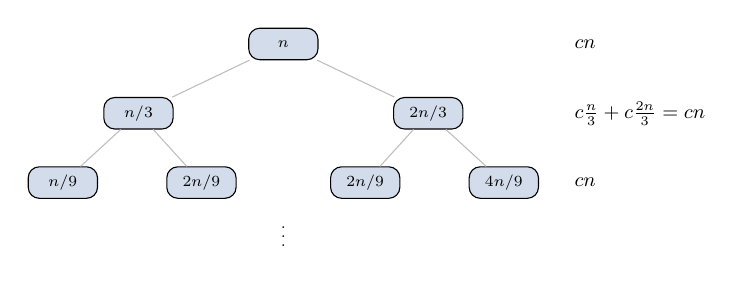
\begin{tikzpicture}[scale=0.80, every node/.style={transform shape},
      lv/.style={draw, rounded corners, fill=mLightBlue!25, minimum width=11mm,
                 minimum height=5mm, inner sep=1pt}]
    \node[lv] (a)  at (0,0)       {\scriptsize $n$};
    \node[lv] (b1) at (-2.3,-1.1) {\scriptsize $n/3$};
    \node[lv] (b2) at (2.3,-1.1)  {\scriptsize $2n/3$};
    \node[lv] (c1) at (-3.5,-2.2) {\scriptsize $n/9$};
    \node[lv] (c2) at (-1.3,-2.2) {\scriptsize $2n/9$};
    \node[lv] (c3) at (1.3,-2.2)  {\scriptsize $2n/9$};
    \node[lv] (c4) at (3.5,-2.2)  {\scriptsize $4n/9$};
    \draw[mGray] (a) -- (b1);  \draw[mGray] (a) -- (b2);
    \draw[mGray] (b1) -- (c1); \draw[mGray] (b1) -- (c2);
    \draw[mGray] (b2) -- (c3); \draw[mGray] (b2) -- (c4);
    \node at (0,-2.95) {\scriptsize $\vdots$};
    \node[right] at (4.5,0)    {\small $cn$};
    \node[right] at (4.5,-1.1) {\small $c\frac{n}{3} + c\frac{2n}{3} = cn$};
    \node[right] at (4.5,-2.2) {\small $cn$};
  \end{tikzpicture}
  \end{center}

  Since $\tfrac13 + \tfrac23 = 1$, every full level costs $cn$. The tree is
  lopsided: its shallowest leaf sits at depth $\log_3 n$ and its deepest at
  $\log_{3/2} n$, both $\Theta(\log n)$.

  \answer{$T(n) = \Theta(n \log n)$}
\end{frame}

% ------------------------------------------------------------------- Q3
\begin{frame}{Q3}
  \begin{center}
    \Large
    Solve \quad $T(n) = T(n/10) + O(n^2)$.
  \end{center}
\end{frame}

\begin{frame}{Q3: Solution}
  Master theorem with
  \[
    a = 1, \qquad b = 10, \qquad d = 2,
    \qquad \log_{10} 1 = 0.
  \]

  \bigskip
  Since $d = 2 > 0 = \log_b a$, the \alert{root dominates}.

  \bigskip
  Sanity check by unrolling: the work per level is
  \[
    cn^2,\;\; c\left(\frac{n}{10}\right)^{2},\;\; c\left(\frac{n}{100}\right)^{2},\ldots
    \;=\; cn^2\left(1 + \frac{1}{100} + \frac{1}{100^2} + \cdots\right)
    \;\le\; \frac{100}{99}\, cn^2 .
  \]

  \answer{$T(n) = O(n^2)$}
\end{frame}

% ------------------------------------------------------------------- Q4
\begin{frame}[fragile]{Q4}
  What is the worst-case running time recurrence for this algorithm?

  \begin{lstlisting}
Function foo(a[1:n], x)
    If n < 10:
        return a[1] + a[2] + ... + a[n] - x

    If a[n] > 10:
        y = 0
        for i = 1, 2, ..., n/3:
            y = y + a[i]
        return foo(a[1:n/3], y)
    else:
        return a[1] + a[2] + ... + a[n] + x * x
  \end{lstlisting}
\end{frame}

\begin{frame}{Q4: Solution}
  Work through the branches.

  \begin{itemize}
    \item \textbf{Base case} $n < 10$: a constant amount of work, $O(1)$.
    \item \textbf{else branch}: summing $a[1 \ldots n]$ costs $O(n)$, no recursion.
    \item \textbf{if branch}: the loop runs $n/3$ times at $O(1)$ each, so $O(n)$,
          followed by \alert{one} recursive call on $n/3$ elements.
  \end{itemize}

  \bigskip
  The worst case is the branch that recurses:

  \answer{$T(n) = T(n/3) + O(n)$, \quad which solves to $T(n) = O(n)$.}

  \bigskip
  \begin{center}
    \small One subproblem of a third the size, so the work shrinks
    geometrically and the root dominates.
  \end{center}
\end{frame}

% =========================================================================
\section{True or False}

% ------------------------------------------------------------------- Q5
\begin{frame}{Q5}
  \begin{center}
    \Large
    $3^n = O(2^n)$. \quad True or false?
  \end{center}
\end{frame}

\begin{frame}{Q5: Solution}
  \begin{center}
    \alert{\Large False.}
  \end{center}

  \bigskip
  For $3^n = O(2^n)$ we would need a constant $c$ with $3^n \le c \cdot 2^n$
  for all large $n$, that is
  \[
    \left(\frac{3}{2}\right)^{n} \le c .
  \]

  \bigskip
  But $\displaystyle \lim_{n \to \infty} \frac{3^n}{2^n}
  = \lim_{n \to \infty}\left(\frac32\right)^{n} = \infty$,
  so no such constant exists.

  \bigskip
  \begin{center}
    In fact $3^n = \omega(2^n)$: different bases are \alert{not} interchangeable.
  \end{center}
\end{frame}

% ------------------------------------------------------------------- Q6
\begin{frame}{Q6}
  \begin{center}
    \Large
    $1^{10} + 2^{10} + 3^{10} + \cdots + n^{10} = \Theta(n^{10})$.\\[0.6em]
    True or false?
  \end{center}
\end{frame}

\begin{frame}{Q6: Solution}
  \begin{center}
    \alert{\Large False.} \quad It is $\Theta(n^{11})$.
  \end{center}


\end{frame}

% =========================================================================
\section{Shortest Paths in a DAG}

% ------------------------------------------------------------------- Q7
\begin{frame}{Q7}
  The vertices $v_1, \ldots, v_6$ are in topological order, so every edge goes
  left to right. Edge lengths may be \alert{negative}.

  \begin{center}
  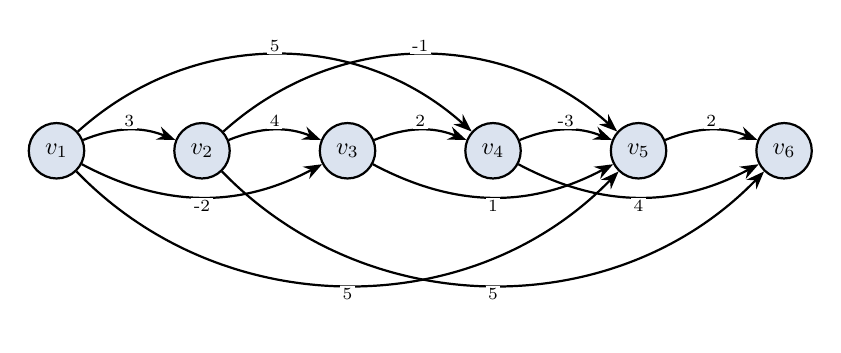
\begin{tikzpicture}[scale=0.88, every node/.style={transform shape},
      >=Stealth, thick,
      vtx/.style={circle, draw, minimum size=8mm, inner sep=1pt, fill=mLightBlue!20},
      lbl/.style={draw=none, fill=white, inner sep=1pt, font=\scriptsize}]
    \foreach \i in {1,...,6} \node[vtx] (v\i) at (2.1*\i - 2.1, 0) {$v_\i$};
    % span 1 (above, small)
    \draw[->] (v1) to[bend left=22] node[lbl, above] {3}  (v2);
    \draw[->] (v2) to[bend left=22] node[lbl, above] {4}  (v3);
    \draw[->] (v3) to[bend left=22] node[lbl, above] {2}  (v4);
    \draw[->] (v4) to[bend left=22] node[lbl, above] {-3} (v5);
    \draw[->] (v5) to[bend left=22] node[lbl, above] {2}  (v6);
    % span 2 (below)
    \draw[->] (v1) to[bend right=28] node[lbl, below] {-2} (v3);
    \draw[->] (v3) to[bend right=28] node[lbl, below] {1}  (v5);
    \draw[->] (v4) to[bend right=28] node[lbl, below] {4}  (v6);
    % span 3 (above, tall)
    \draw[->] (v1) to[bend left=42] node[lbl, above] {5}  (v4);
    \draw[->] (v2) to[bend left=42] node[lbl, above] {-1} (v5);
    % span 4 (below, deep)
    \draw[->] (v1) to[bend right=46] node[lbl, below] {5} (v5);
    \draw[->] (v2) to[bend right=46] node[lbl, below] {5} (v6);
  \end{tikzpicture}
  \end{center}

  \begin{center}
    Compute the shortest path length from $v_1$ to each of
    $v_2, \ldots, v_6$.
  \end{center}
\end{frame}

\begin{frame}{Q7: Solution}
  Fill left to right using
  $\;dist[v_j] = \min_{v_i \to v_j} \big( dist[v_i] + W[v_i, v_j] \big)$.

  \bigskip
  \begin{itemize}\small
    \item $dist[v_2] = 0 + 3 = 3$
    \item $dist[v_3] = \min(\underbrace{0 - 2}_{v_1},\; \underbrace{3 + 4}_{v_2}) = -2$
    \item $dist[v_4] = \min(\underbrace{0 + 5}_{v_1},\; \underbrace{-2 + 2}_{v_3}) = 0$
    \item $dist[v_5] = \min(\underbrace{0 + 5}_{v_1},\; \underbrace{3 - 1}_{v_2},\;
                            \underbrace{-2 + 1}_{v_3},\; \underbrace{0 - 3}_{v_4}) = -3$
    \item $dist[v_6] = \min(\underbrace{3 + 5}_{v_2},\; \underbrace{0 + 4}_{v_4},\;
                            \underbrace{-3 + 2}_{v_5}) = -1$
  \end{itemize}

  \answer{$dist = [\,0,\; 3,\; -2,\; 0,\; -3,\; -1\,]$ for $v_1, \ldots, v_6$}
\end{frame}

\begin{frame}{Q7: The Shortest Path Tree}
  \begin{center}
  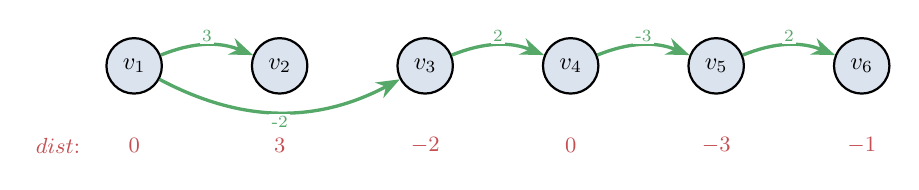
\begin{tikzpicture}[scale=0.88, every node/.style={transform shape},
      >=Stealth, thick,
      vtx/.style={circle, draw, minimum size=8mm, inner sep=1pt, fill=mLightBlue!20},
      lbl/.style={draw=none, fill=white, inner sep=1pt, font=\scriptsize}]
    \foreach \i in {1,...,6} \node[vtx] (v\i) at (2.1*\i - 2.1, 0) {$v_\i$};
    \foreach \i/\d in {1/0, 2/3, 3/-2, 4/0, 5/-3, 6/-1}
      \node[mRed] at (2.1*\i - 2.1, -1.15) {\small $\d$};
    \draw[->, mGreen, very thick] (v1) to[bend left=22] node[lbl, above] {3}  (v2);
    \draw[->, mGreen, very thick] (v3) to[bend left=22] node[lbl, above] {2}  (v4);
    \draw[->, mGreen, very thick] (v4) to[bend left=22] node[lbl, above] {-3} (v5);
    \draw[->, mGreen, very thick] (v5) to[bend left=22] node[lbl, above] {2}  (v6);
    \draw[->, mGreen, very thick] (v1) to[bend right=28] node[lbl, below] {-2} (v3);
    \node[mRed] at (-1.1,-1.15) {\small $dist$:};
  \end{tikzpicture}
  \end{center}

  \bigskip
  \begin{center}
  \begin{tabular}{ll}
    \toprule
    target & shortest path \\
    \midrule
    $v_2$ & $v_1 \to v_2$ \hfill $3$ \\
    $v_3$ & $v_1 \to v_3$ \hfill $-2$ \\
    $v_4$ & $v_1 \to v_3 \to v_4$ \hfill $0$ \\
    $v_5$ & $v_1 \to v_3 \to v_4 \to v_5$ \hfill $-3$ \\
    $v_6$ & $v_1 \to v_3 \to v_4 \to v_5 \to v_6$ \hfill $-1$ \\
    \bottomrule
  \end{tabular}
  \end{center}
\end{frame}

% =========================================================================
\section{Reading DP Tables}

% ------------------------------------------------------------------- Q8
\begin{frame}{Q8}
  Let $K[i,c]$ be the maximum value using items $1, \ldots, i$ with capacity $c$.
  Suppose

  \begin{center}
  \begin{tabular}{llll}
    $K[149, 400] = 910$ & $K[149, 280] = 700$ & $K[148, 400] = 880$ & $w[150] = 120$ \\
    $K[149, 120] = 310$ & $K[149, 250] = 640$ & $K[100, 200] = 450$ & $v[150] = 260$ \\
    $K[148, 280] = 690$ & $K[149, 300] = 760$ & $w[125] = 75$       & $v[125] = 140$ \\
  \end{tabular}
  \end{center}

  \bigskip
  \begin{center}
    \Large What is $K[150, 400]$?
  \end{center}
\end{frame}

\begin{frame}{Q8: Solution}
  The recurrence looks only at row $i-1$:
  \[
    K[i,c] = \max\big( \underbrace{K[i-1,c]}_{\text{skip item } i},\;
                       \underbrace{K[i-1,\, c - w[i]] + v[i]}_{\text{take item } i} \big).
  \]

  \bigskip
  With $i = 150$, $c = 400$, $w[150] = 120$, $v[150] = 260$:
  \[
    K[150,400] = \max\big( K[149,400],\; K[149,\, 400-120] + 260 \big)
               = \max\big( 910,\; 700 + 260 \big).
  \]

  \answer{$K[150,400] = \max(910,\; 960) = \mathbf{960}$ \quad (take item $150$)}

  \bigskip
  \begin{center}
    \small Everything else listed is a distractor: rows other than $149$ and
    capacities other than $400$ and $280$ never appear.
  \end{center}
\end{frame}

% ------------------------------------------------------------------- Q9
\begin{frame}{Q9}
  Let $ED[i,j]$ be the edit distance between $A[1 \ldots i]$ and
  $B[1 \ldots j]$. Suppose $A[7] = \texttt{T}$ and $B[5] = \texttt{T}$, and

  \begin{center}
  \begin{tabular}{llll}
    $ED[6,5] = 8$ & $ED[7,4] = 6$ & $ED[6,4] = 5$ & $ED[5,5] = 9$ \\
    $ED[7,3] = 11$ & $ED[6,6] = 7$ & $ED[5,4] = 4$ & $ED[7,6] = 9$ \\
  \end{tabular}
  \end{center}

  \bigskip
  \begin{center}
    \Large What is $ED[7,5]$?
  \end{center}
\end{frame}

\begin{frame}{Q9: Solution}
  \[
    ED[i,j] = \min\big(
      \underbrace{ED[i-1,j] + 1}_{\text{delete } A[i]},\;
      \underbrace{ED[i,j-1] + 1}_{\text{insert } B[j]},\;
      \underbrace{ED[i-1,j-1] + \text{diff}(i,j)}_{\text{substitute}} \big).
  \]

  \bigskip
  Since $A[7] = B[5] = \texttt{T}$, we have $\text{diff}(7,5) = \alert{0}$.
  So
  \[
    ED[7,5] = \min\big( \underbrace{8+1}_{ED[6,5]},\;
                        \underbrace{6+1}_{ED[7,4]},\;
                        \underbrace{5+0}_{ED[6,4]} \big).
  \]

  \answer{$ED[7,5] = \min(9,\, 7,\, 5) = \mathbf{5}$ \quad (characters match, so no edit)}
\end{frame}

% =========================================================================
\section{Majority Element}

% ------------------------------------------------------------------- Q10
\begin{frame}{Q10}
  Let $L, R$ be a partition of $A[1:n]$.

  \bigskip
  \begin{center}
    \Large
    If $x$ is the majority of $L$, then $x$ is always the majority of $A$.\\[0.6em]
    True or false?
  \end{center}
\end{frame}

\begin{frame}{Q10: Solution}
  \begin{center}
    \alert{\Large False.}
  \end{center}

  \bigskip
  \textbf{Counterexample.} Take $L = [a, a]$ and $R = [b, b, b, b]$.

  \begin{center}
  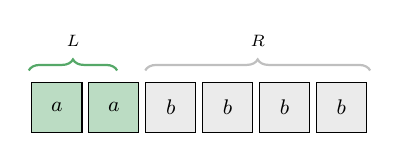
\begin{tikzpicture}[scale=0.85, every node/.style={transform shape}]
    \foreach \v/\fc [count=\i from 0] in
      {a/mGreen!40, a/mGreen!40, b/black!8, b/black!8, b/black!8, b/black!8}
      \node[draw, minimum size=7.5mm, fill=\fc] at (\i*0.85,0) {\small $\v$};
    \draw[decorate, decoration={brace, amplitude=4pt}, mGreen, thick]
      (-0.42,0.55) -- (0.9,0.55);
    \node[above] at (0.24,0.78) {\scriptsize $L$};
    \draw[decorate, decoration={brace, amplitude=4pt}, mGray, thick]
      (1.32,0.55) -- (4.68,0.55);
    \node[above] at (3.0,0.78) {\scriptsize $R$};
  \end{tikzpicture}
  \end{center}

  \bigskip
  $a$ occurs twice in $L$, and $2 > |L|/2 = 1$, so $a$ \alert{is} the majority
  of $L$.

  \bigskip
  But in $A$ it occurs $2$ times out of $n = 6$, and $2 \not> 3$. So $a$ is
  \alert{not} the majority of $A$.
\end{frame}

% ------------------------------------------------------------------- Q11
\begin{frame}{Q11}
  Let $L, R$ be a partition of $A[1:n]$.

  \bigskip
  \begin{center}
    \Large
    If $x$ is the majority of $L$ \emph{and} the majority of $R$,\\
    then $x$ is always the majority of $A$.\\[0.6em]
    True or false?
  \end{center}
\end{frame}

\begin{frame}{Q11: Solution}
  \begin{center}
    \alert{\Large True.}
  \end{center}

  \bigskip
  By assumption,
  \[
    \text{count}(x, L) > \frac{|L|}{2}
    \qquad\text{and}\qquad
    \text{count}(x, R) > \frac{|R|}{2}.
  \]

  \bigskip
  Adding the two inequalities,
  \[
    \text{count}(x, A) = \text{count}(x,L) + \text{count}(x,R)
    \;>\; \frac{|L| + |R|}{2} = \frac{n}{2}.
  \]

  \bigskip
  \begin{center}
    So $x$ occurs strictly more than $n/2$ times in $A$. $\square$
  \end{center}

  \bigskip
  \begin{center}
    \small Compare with Q10: one half is not enough, but both halves is.
  \end{center}
\end{frame}

% =========================================================================
\section{Algorithm Design}

% ------------------------------------------------------------------- Q12
\begin{frame}{Q12}
  A sorted array $A[1:n]$ of \textbf{distinct} elements has been cyclically
  shifted $k$ positions to the right. Find $k$ in $O(\log n)$ time.

  \bigskip
  \begin{center}
  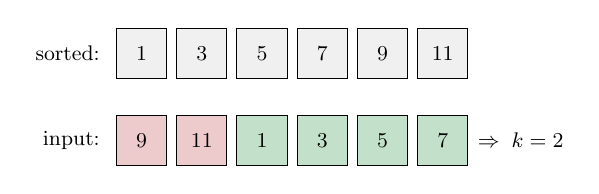
\begin{tikzpicture}[scale=0.85, every node/.style={transform shape}]
    \node[left] at (-0.5,0.8) {\small sorted:};
    \foreach \v [count=\i from 0] in {1,3,5,7,9,11}
      \node[draw, minimum size=7.5mm, fill=black!6] at (\i*0.9,0.8) {\small \v};
    \node[left] at (-0.5,-0.5) {\small input:};
    \foreach \v/\fc [count=\i from 0] in
      {9/mRed!30, 11/mRed!30, 1/mGreen!35, 3/mGreen!35, 5/mGreen!35, 7/mGreen!35}
      \node[draw, minimum size=7.5mm, fill=\fc] at (\i*0.9,-0.5) {\small \v};
    \node[right] at (4.9,-0.5) {\small $\Rightarrow\; k = 2$};
  \end{tikzpicture}
  \end{center}

  \bigskip
  \begin{center}
    \small The last $k$ elements have wrapped around to the front.
  \end{center}
\end{frame}

\begin{frame}{Q12: Solution}
  \textbf{Key observation.} The array is two sorted runs, and the
  \alert{minimum} sits at index $k+1$. So finding $k$ means finding the
  minimum's index.

  \bigskip
  Compare $A[\textit{mid}]$ against the \alert{last} element $A[\textit{hi}]$:

  \begin{itemize}
    \item $A[\textit{mid}] > A[\textit{hi}]$: the wrap point is to the
          \emph{right}, so search $[\textit{mid}+1, \textit{hi}]$.
    \item otherwise: $\textit{mid}$ is in the second run, so the minimum is at
          $\textit{mid}$ or to its left, search $[\textit{lo}, \textit{mid}]$.
  \end{itemize}

  \bigskip
  \begin{center}
  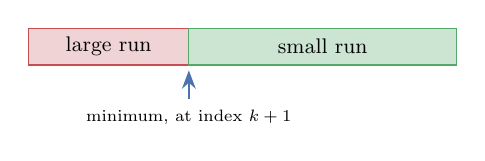
\begin{tikzpicture}[scale=0.85, every node/.style={transform shape}]
    \fill[mRed!25, draw=mRed] (0,0) rectangle (2.4,0.55);
    \fill[mGreen!30, draw=mGreen] (2.4,0) rectangle (6.4,0.55);
    \node at (1.2,0.28) {\small large run};
    \node at (4.4,0.28) {\small small run};
    \draw[-{Stealth}, thick, mLightBlue] (2.4,-0.5) -- (2.4,-0.08);
    \node[below] at (2.4,-0.55) {\scriptsize minimum, at index $k+1$};
  \end{tikzpicture}
  \end{center}
\end{frame}

\begin{frame}[fragile]{Q12: Solution}
  \begin{lstlisting}
# Index of the minimum inside A[lo:hi]
function min_index(A, lo, hi)
    if lo == hi
        return lo                          # base case: one element left
    end

    mid = div(lo + hi, 2)
    if A[mid] > A[hi]
        return min_index(A, mid + 1, hi)   # wrap point is to the right
    else
        return min_index(A, lo, mid)       # minimum is at mid or left of it
    end
end

find_shift(A) = min_index(A, 1, length(A)) - 1
  \end{lstlisting}

  \bigskip
  Each call discards half the range, so
  $T(n) = T(n/2) + O(1) = O(\log n)$ by the Master theorem.
\end{frame}


% ------------------------------------------------------------------- Q13
\begin{frame}{Q13}
  The 0-1 knapsack problem with values $v[1:n]$, weights $w[1:n]$, and capacity
  $W$, plus one extra constraint:

  \bigskip
  \begin{center}
    \alert{at most $k$ items may be selected.}
  \end{center}

  \bigskip
  Design a dynamic programming algorithm that outputs the maximum achievable
  value.
\end{frame}

\begin{frame}{Q13: Solution}
  Add a \alert{third dimension} counting how many items we have used.

  \begin{block}{Definition}
    $K[i, c, j]$ = maximum value using items $1 \ldots i$, capacity $c$, and at
    most $j$ items.
  \end{block}

  \bigskip
  The same two choices as before, but taking an item now also spends one of the
  $j$ slots:
  \[
    K[i,c,j] = \max\big(
      \underbrace{K[i-1,\, c,\, j]}_{\text{skip } i},\;
      \underbrace{K[i-1,\; c-w[i],\; j-1] + v[i]}_{\text{take } i,\ \text{if } w[i] \le c,\ j \ge 1}
    \big).
  \]

  \bigskip
  Base cases: $K[0,c,j] = 0$ and $K[i,c,0] = 0$.
\end{frame}

\begin{frame}{Q13: Solution}


  The answer is $K[n, W, k]$.

  \answer{$O(nWk)$ time and $O(nWk)$ space (reducible to $O(Wk)$ by keeping only row $i-1$).}


\end{frame}


% ------------------------------------------------------------------- Q14
\begin{frame}{Q14: Vasya's Vacation}
  Vasya has $n$ vacation days. For day $i$ one of four things holds:

  \begin{center}
  \begin{tabular}{cll}
    \toprule
    $a_i$ & gym & contest \\
    \midrule
    $0$ & closed & no \\
    $1$ & closed & yes \\
    $2$ & open   & no \\
    $3$ & open   & yes \\
    \bottomrule
  \end{tabular}
  \end{center}

  \bigskip
  Each day he rests, writes the contest (if held), or does sport (if the gym is
  open). He will \alert{not repeat the same activity on two consecutive days}.

  \bigskip
  \begin{center}
    Minimise the number of rest days.
  \end{center}
\end{frame}

\begin{frame}{Q14: Solution}
  The only thing that constrains tomorrow is \alert{what he did today}. So make
  that the state.

  \begin{block}{Definition}
    $dp[i][s]$ = fewest rest days over days $1 \ldots i$, where day $i$ ended
    with activity $s \in \{\text{rest}, \text{contest}, \text{sport}\}$.
  \end{block}

  \bigskip
  \begin{align*}
    dp[i][\text{rest}]    &= 1 + \min\big( dp[i-1][\cdot] \big) \\
    dp[i][\text{contest}] &= \min\big( dp[i-1][\text{rest}],\, dp[i-1][\text{sport}] \big)
                             && \text{if } a_i \in \{1,3\} \\
    dp[i][\text{sport}]   &= \min\big( dp[i-1][\text{rest}],\, dp[i-1][\text{contest}] \big)
                             && \text{if } a_i \in \{2,3\}
  \end{align*}

  \bigskip
  Unavailable options are $+\infty$. Answer: $\min_s dp[n][s]$, in $O(n)$ time.
\end{frame}

\begin{frame}{Q14: Example}
  $a = [\,1,\; 3,\; 2,\; 0,\; 3,\; 3,\; 1\,]$

  \bigskip
  \begin{center}
  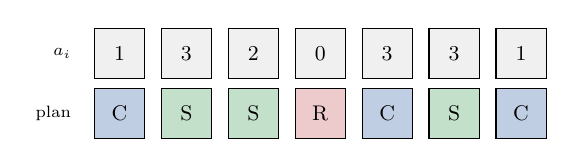
\begin{tikzpicture}[scale=0.85, every node/.style={transform shape}]
    \foreach \v/\act/\fc [count=\i from 0] in
      {1/C/mLightBlue!35, 3/S/mGreen!35, 2/S/mGreen!35, 0/R/mRed!30,
       3/C/mLightBlue!35, 3/S/mGreen!35, 1/C/mLightBlue!35} {
      \node[draw, minimum size=7.5mm, fill=black!6] at (\i*1.0,0.6) {\small \v};
      \node[draw, minimum size=7.5mm, fill=\fc] at (\i*1.0,-0.3) {\small \act};
    }
    \node[left] at (-0.6,0.6)  {\scriptsize $a_i$};
    \node[left] at (-0.6,-0.3) {\scriptsize plan};
  \end{tikzpicture}
  \end{center}

  \bigskip
  \begin{center}
    \small C = contest, \; S = sport, \; R = rest
  \end{center}

  \bigskip
  Day $4$ has $a_4 = 0$, so it is a forced rest. Everything else alternates
  legally.

  \answer{Minimum rest days $= \mathbf{2}$}
\end{frame}

% ------------------------------------------------------------------- Q15
\begin{frame}{Q15: One Flip}
  Given $a_1, \ldots, a_n$ with each $a_i \in \{0, 1\}$, choose indices
  $i \le j$ and flip every $a_k$ with $i \le k \le j$
  (that is $x \mapsto 1 - x$).

  \bigskip
  \begin{center}
    You must make \alert{exactly one} move. Maximise the number of ones.
  \end{center}

  \bigskip
  \begin{center}
  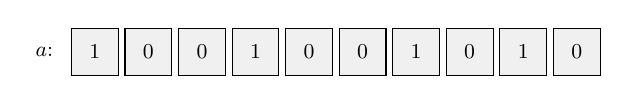
\begin{tikzpicture}[scale=0.85, every node/.style={transform shape}]
    \foreach \v [count=\i from 0] in {1,0,0,1,0,0,1,0,1,0}
      \node[draw, minimum size=7mm, fill=black!6] at (\i*0.8,0) {\small \v};
    \node[left] at (-0.5,0) {\small $a$:};
  \end{tikzpicture}
  \end{center}
\end{frame}

\begin{frame}{Q15: Solution}
  Flipping the range $[i,j]$ turns its zeros into ones and its ones into zeros,
  so
  \[
    \text{ones after} = \text{(total ones)} \;-\; \text{ones in } [i,j]
                        \;+\; \text{zeros in } [i,j].
  \]

  \bigskip
  Define
  \[
    b_k = \begin{cases} +1 & \text{if } a_k = 0, \\ -1 & \text{if } a_k = 1. \end{cases}
  \]
  Then the gain from flipping $[i,j]$ is exactly $\sum_{k=i}^{j} b_k$.

  \bigskip
  \begin{alertblock}{}
    The answer is $\;\text{(total ones)} + \big(\text{maximum subarray sum of } b\big)$,
    over \alert{non-empty} subarrays.
  \end{alertblock}

  \bigskip
  Kadane's algorithm gives this in $O(n)$.
\end{frame}

\begin{frame}{Q15: Example}
  \begin{center}
  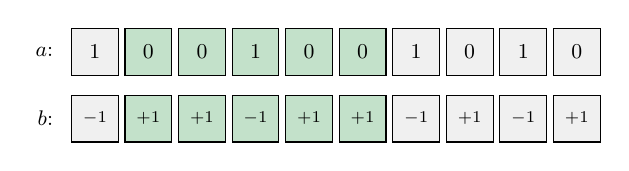
\begin{tikzpicture}[scale=0.85, every node/.style={transform shape}]
    \node[left] at (-0.5,0.6) {\small $a$:};
    \foreach \v/\fc [count=\i from 0] in
      {1/black!6, 0/mGreen!35, 0/mGreen!35, 1/mGreen!35, 0/mGreen!35,
       0/mGreen!35, 1/black!6, 0/black!6, 1/black!6, 0/black!6}
      \node[draw, minimum size=7mm, fill=\fc] at (\i*0.8,0.6) {\small \v};
    \node[left] at (-0.5,-0.4) {\small $b$:};
    \foreach \v/\fc [count=\i from 0] in
      {$-$1/black!6, $+$1/mGreen!35, $+$1/mGreen!35, $-$1/mGreen!35, $+$1/mGreen!35,
       $+$1/mGreen!35, $-$1/black!6, $+$1/black!6, $-$1/black!6, $+$1/black!6}
      \node[draw, minimum size=7mm, fill=\fc, font=\scriptsize] at (\i*0.8,-0.4) {\v};
  \end{tikzpicture}
  \end{center}

  \bigskip
  Total ones $= 4$. The best subarray of $b$ is positions $2 \ldots 6$ with sum
  $1+1-1+1+1 = 3$.

  \answer{Maximum ones $= 4 + 3 = \mathbf{7}$}

  \bigskip
  \begin{center}
    \small Watch the edge case: if $a$ is all ones, the move still has to
    happen, so the answer is $(\text{total ones}) - 1$.
  \end{center}
\end{frame}

% ------------------------------------------------------------------- Q16
\begin{frame}{Q16: Vitamins}
  A shop sells $n$ juices. Juice $i$ costs $c_i$ and contains some non-empty
  subset of the vitamins $\{A, B, C\}$.

  \bigskip
  \begin{center}
    What is the minimum total price to obtain \alert{all three} vitamins?\\
    Return $-1$ if it is impossible.
  \end{center}

  \bigskip
  \begin{center}
  \begin{tabular}{lcccc}
    \toprule
    juice    & 1 & 2 & 3 & 4 \\
    \midrule
    price    & $5$ & $6$ & $16$ & $4$ \\
    vitamins & \texttt{C} & \texttt{B} & \texttt{BAC} & \texttt{A} \\
    \bottomrule
  \end{tabular}
  \end{center}
\end{frame}

\begin{frame}{Q16: Solution}
  Only the \alert{set} of vitamins matters, and there are just
  $2^3 = 8$ subsets. Encode each juice as a 3-bit mask.

  \begin{block}{Definition}
    $dp[\textit{mask}]$ = minimum cost to obtain exactly the vitamins in
    $\textit{mask}$ (or better).
  \end{block}

  \bigskip
  Start with $dp[000] = 0$ and everything else $+\infty$. For each juice with
  mask $m$ and price $c$, and every $s$:
  \[
    dp[\,s \,|\, m\,] \;\leftarrow\; \min\big( dp[\,s \,|\, m\,],\; dp[s] + c \big).
  \]

  \bigskip
  The answer is $dp[111]$, or $-1$ if it is still $+\infty$.

  \answer{$O(n \cdot 2^3) = O(n)$ time}
\end{frame}

\begin{frame}{Q16: Example}
  \begin{center}
  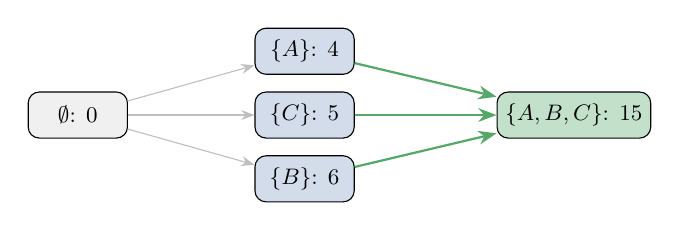
\begin{tikzpicture}[scale=0.9, every node/.style={transform shape},
      st/.style={draw, rounded corners, minimum width=14mm, minimum height=6.5mm,
                 font=\small}]
    \node[st, fill=black!6]     (e)  at (0,0)     {$\emptyset$: $0$};
    \node[st, fill=mLightBlue!25] (a) at (3.2,0.9)  {$\{A\}$: $4$};
    \node[st, fill=mLightBlue!25] (c) at (3.2,0)    {$\{C\}$: $5$};
    \node[st, fill=mLightBlue!25] (b) at (3.2,-0.9) {$\{B\}$: $6$};
    \node[st, fill=mGreen!35]   (all) at (7.0,0)   {$\{A,B,C\}$: $15$};
    \draw[-{Stealth}, mGray] (e) -- (a);
    \draw[-{Stealth}, mGray] (e) -- (c);
    \draw[-{Stealth}, mGray] (e) -- (b);
    \draw[-{Stealth}, thick, mGreen] (a) -- (all);
    \draw[-{Stealth}, thick, mGreen] (c) -- (all);
    \draw[-{Stealth}, thick, mGreen] (b) -- (all);
  \end{tikzpicture}
  \end{center}

  \bigskip
  Buying the three single-vitamin juices costs $4 + 5 + 6 = 15$, which beats the
  all-in-one juice at $16$.

  \answer{Minimum total price $= \mathbf{15}$}
\end{frame}

\end{document}
